%&latex

\documentclass[conference]{IEEEtran}
\usepackage[cmex10]{amsmath}
\usepackage{algorithmic}
\usepackage{array}
\usepackage{eqparbox}
\usepackage[english]{babel}
% *** SUBFIGURE PACKAGES ***


\usepackage{graphicx}
\usepackage{epsfig}
\usepackage{epstopdf}
\usepackage{amsmath} 
%\usepackage[caption=false]{caption}
\usepackage[font=footnotesize]{subfig}
\usepackage{stfloats}
\usepackage{float}
\usepackage{subfig}
\usepackage{amssymb}
\usepackage{cite} 
\usepackage[T1]{fontenc}
%\usepackage{hyperref}
\begin{document}

\title{Proyecto de Investigación de cotizador automático por medio de ChatBots}
\author
{
\IEEEauthorblockN{D.~Figueroa-Castañeda}\\
\IEEEauthorblockA
{
	Universidad Interamericana~ Maestría en automatización industrial, \\manufactura 		digital, y robótica\\
	Puebla,~Mexico \\
	email: \{d.figueroa@lainter.edu.mx}
}



% The paper headers
\markboth{}%
{Shell \MakeLowercase{\textit{et al.}}: Bare Demo of IEEEtran.cls for Journals}

% make the title area
\maketitle


 
\begin{abstract}
 ~En ésta investigación se abordará la integración de programas con capacidad de interactuar por medio de texto con usuarios humanos, conocidos como ChatBot's, para la automatización del proceso de cotización de productos y servicios a través de Internet, en específico, del servicio de Impresión 3D y manufactura aditiva. A través de la creación de un ChatBot para interacuar en Telegram y Facebook desarrollado en Node-RED, una plataforma de programación visual que permite integrar diferentes servicios WEB a través de API's y control de Hardware facilmente, permitiendo administrar también el flujo de trabajo de una granja de impresoras 3D.
\end{abstract}
\vspace{0.5cm}
\textbf{Keywords}:  ChatBot, Node-RED, Cotizador automático, Impresión 3D.

\IEEEpeerreviewmaketitle
\section{Introduccion}
\IEEEPARstart{A}ctualmente es muy común encontrar procesos donde un programa puede facilmente solventar tareas repetitivas, desde sujetar una pieza y depositarla en un lugar en específico dentro de una linea de producción, hasta contestar el teléfono y agendar una cita como se ha visto en algunos desarrollos de empresas como Google. La situacción actual de confinamiento hace necesario una mayor demanda de servicios a través de internet, exigiendo a muchas empresas a innovar en soluciones que les permita continuar prestando servicios, presindiendo de la fuerza laboral presencial y dando paso a formas de trabajo remoto y en el mejor de los casos más automatizado. Esta investigación se encuentra organizada de la siguiente manera. En la Sección $\mathbf{II}$, se hablará del proceso de impresión 3D y la necesidad de integrar un ChatBot que realice cotizaciones, en la Sección $\mathbf{III}$ se abordará el uso de Node-RED para desarrollar el algoritmo de cotización de la impresión 3D, así como el ChatBot. En la Sección $\mathbf{IV}$ se introduce, la Raspberry Pi 4, como la plataforma donde correrá nuestro programa. Finalmente, las conclusiones son presentadas en la Sección $\mathbf{V}$.

\section{Impresión 3D}

La impresión 3D es un proceso de manufactura aditiva donde se debe considerar el material usado en el proceso, el tiempo necesario para la fabricación así como el volumen final y peso. Adicionalmente es necesaro considerar la energía eléctrica necesaria, material de soportes y un factor de complejidad, con esos parametros, se puede realizar una cotización más adecuada y justa con el cliente final.

\begin{equation}
\label{ohm}
P=T*F*V*E,
\end{equation}

Donde:\\

P = Precio total al cliente.\\
T = Tiempo necesario.\\
F = Factor de complejidad.\\
V = Volumen para empaquetar.\\
E = Energía necesaria.\\

El Factor de complejidad:  
 \begin{equation}
    \label{Homotopia_G}
     F= Resolucion / Area * Altura,
 \end{equation}
 
          
     
La Resolución en impresión 3D, hace referencia al grosor con el que la máquina crea cada capa de los objetos impresos, entre más capas son necesarias es mayor el riesgo de que algo salga mal. Otro punto en contra es el Área de impresión del objeto en comparación a la altura, debido a que si esa proporción es muy alta en comparación con la base, puede generar que la base de la pieza que toca la superficie de la impresora se despegue o que sea más fácil que la boquilla la termine golpeando, haciendo la pieza se desprenda y falle, causando perdida de material y tiempo. 

\begin{figure}[H]
\begin{center}
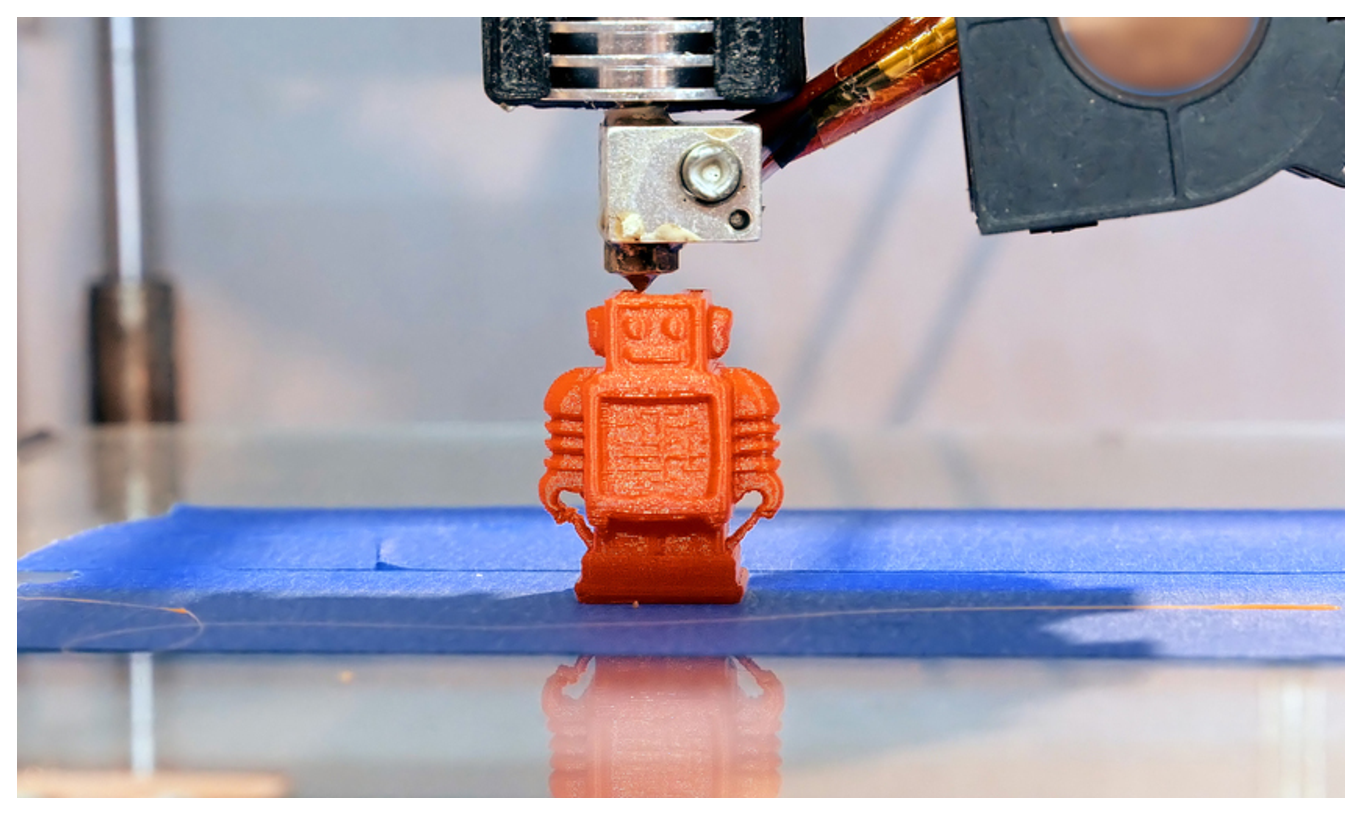
\includegraphics[width=0.2\textwidth]{imagenes/imp3d.eps} 
\caption{ Pieza en impresión 3D.}
\label{fig:hiper2}
\end{center}
\end{figure}   
 
\section{Node-RED}
Existen diferentes paradigmas de programación, uno de los que más terreno ha ganado en estos días ha sido JavaSript por su fácil integración con ambientes web. Tomando como base ese lenguaje se dasarrolló un proyecto denominado Node.JS, donde, se simplifica el modo de programación, generando entornos web, con la posibilidad de comunicarse a través de mensajes o acciones. Por otro lado, han ganado terreno, formas de organizar programas de forma visual, siendo Node-RED, un entorno que junta de manera visual, gran cantidad de librerias, su filosofía se basa en simplificar el funcionamiento de las mismas, reduciendo el desarrollo a enviar un mensaje muy simple, que se puede compartir indistintamente a otras funciones y ser procesado por las mismas, generando un flujo de información que se autodocumenta.

\begin{figure}[H]
\begin{center}
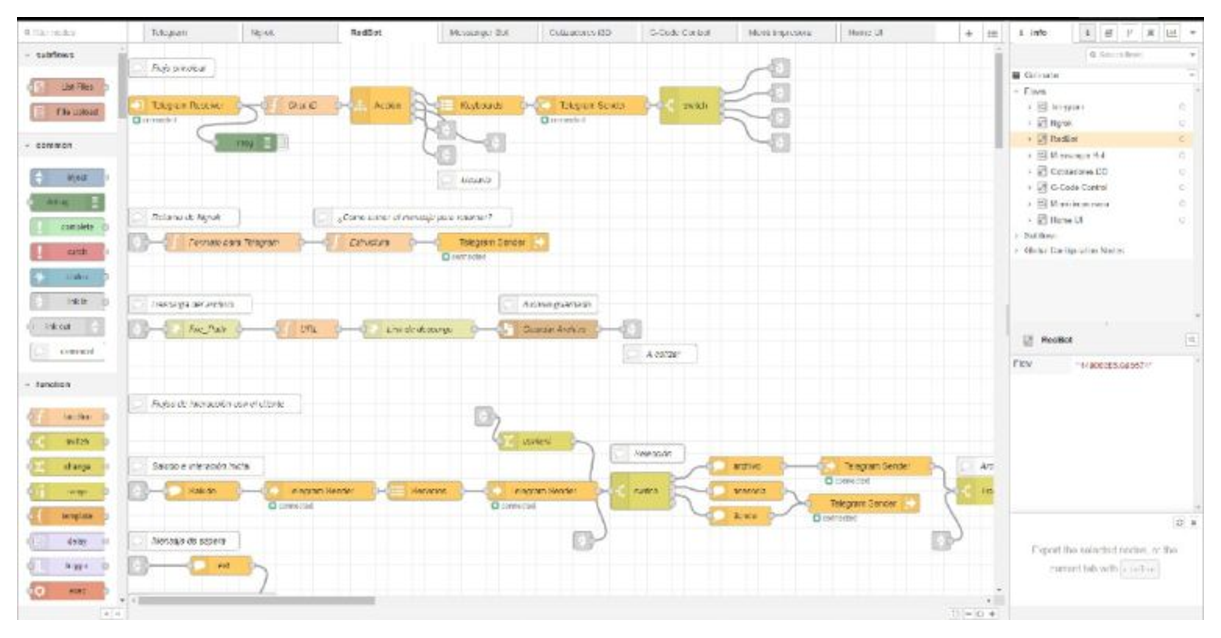
\includegraphics[width=0.2\textwidth]{imagenes/node.eps} 
\caption{ Nodos y Flujos en Node-RED.}
\label{fig:hiper2}
\end{center}
\end{figure}    

%-----------------------------------------------------------------------------------------------------------

\section{Node-RED}
 \begin{figure}[H]
\begin{center}
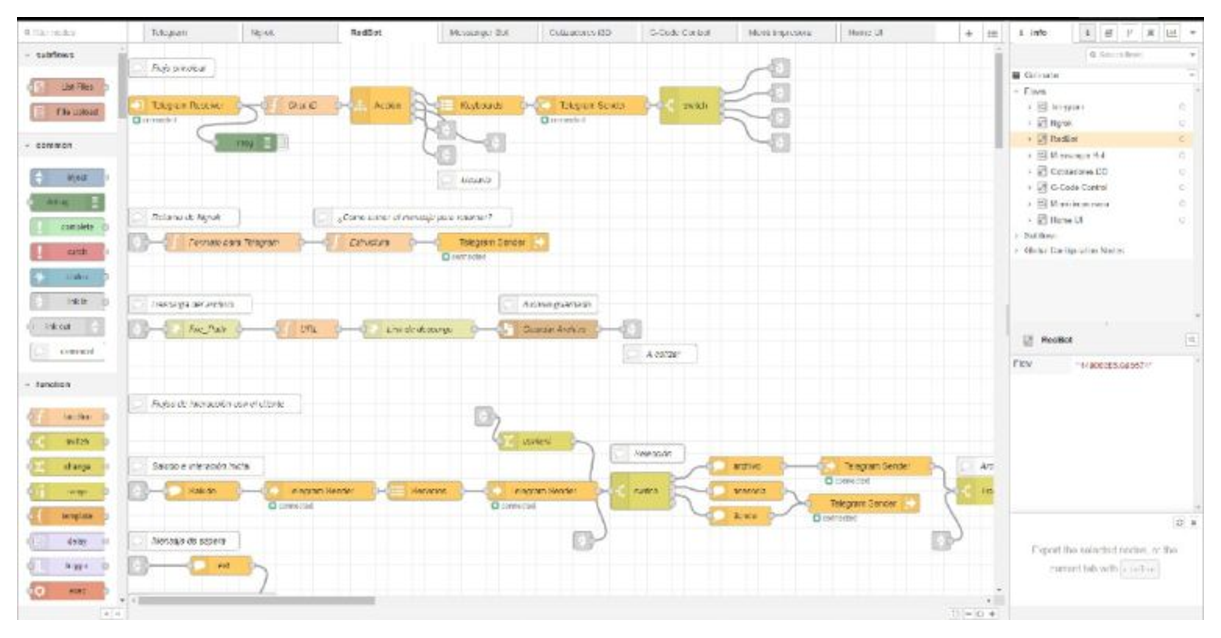
\includegraphics[width=0.2\textwidth]{imagenes/node.eps} 
\caption{ Nodos y Flujos en Node-RED.}
\label{fig:hiper2}
\end{center}
\end{figure}    


  \begin{figure}[H]
\begin{center}
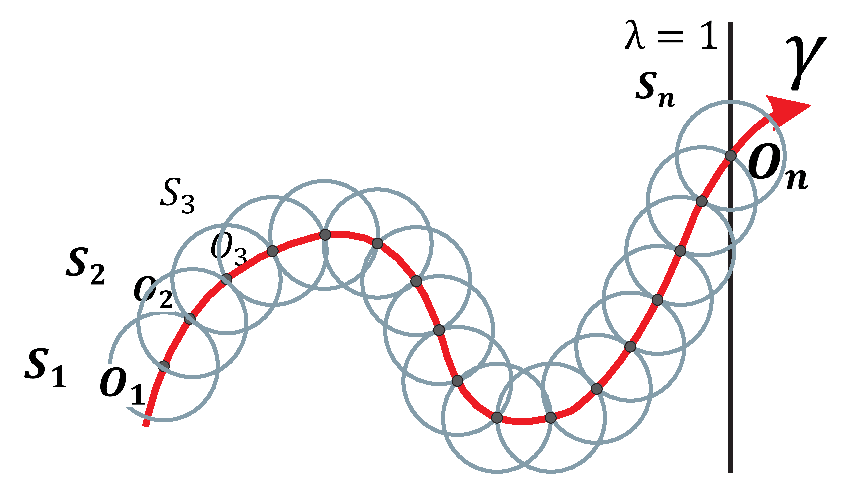
\includegraphics[width=0.2\textwidth]{imagenes/hiper2.eps} 
\caption{ Seguimiento.}
\label{fig:hiper3}
\end{center}
\end{figure}    
  
\begin{figure}[H]
\begin{center}
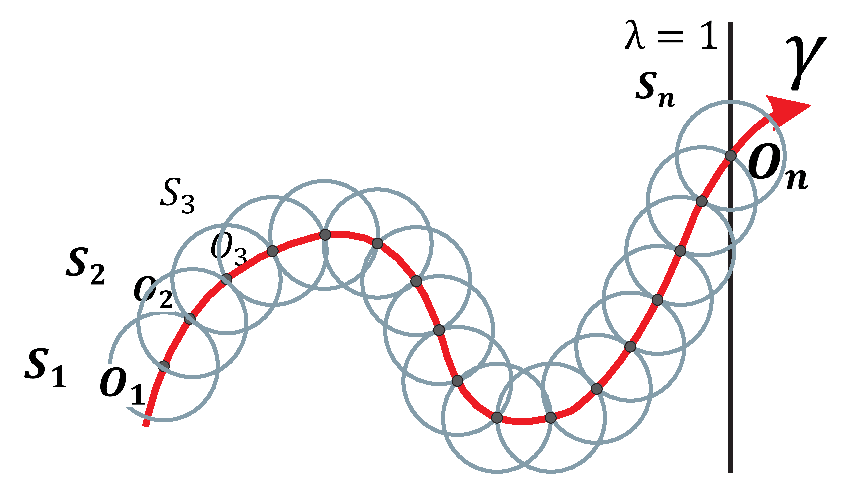
\includegraphics[width=0.2\textwidth]{imagenes/hiper2.eps} 
\caption{ Seguimiento.}
\label{fig:hiper4}
\end{center}
\end{figure}    
  
\subsection*{Predictor-Corrector Scheme}
 A proper \cite{plc1} predictor-corrector Figure \ref{fig:hiper4} scheme \cite{Hector1, Gerardo1}...
  
 
 



\section{Experiments}

The efficiency of the \cite{Park-2008} proposed...
\subsection{Successful path for maps with 200 and 2000 obstacles}

We consider two study cases...

  \vspace{-0.1 cm}
\begin{table}[H]
\begin{center}
\resizebox{9cm}{!} {
\begin{tabular}{ |c|c|c|c|c|c|c|c|c| }
\hline
\multicolumn{9}{|c|}{Environment maps}\\
\hline
\multicolumn{1}{|c}{N.Obstacles}&\multicolumn{4}{|c}{200}&\multicolumn{4}{|c|}{2000}\\
\hline
Path&1&2&3&4&1&2&3&4\\
\hline
Steps&919&898&894&999&7165&6404&7406&6953\\
\hline
Time (ms)&504&483 &504&564&41190&38840&48561&39305\\
\hline
Path length&2.10143&2.06822&2.01062&2.2497&2.59544&2.20463&2.57591&2.40284\\
\hline
\end{tabular}
}
\end{center}
\caption{Computation time and length in normalized units for two environment maps.}
\label{table:tiempos}
\end{table}

%%%jashljdhlsjahlfhsd

\section{Conclusions}
 In this work,...

\bibliographystyle{ieeetr}
\bibliography{bibliography}



\end{document}


